\documentclass[times,twocolumn,final]{elsarticle}

\usepackage{cag}
\usepackage{framed,multirow}
\usepackage{amssymb}
\usepackage{amsmath}
\usepackage{lineno}
\usepackage{graphicx}
\usepackage{booktabs}
\usepackage{placeins}
\setcounter{totalnumber}{6}
\setcounter{topnumber}{4}
\setcounter{bottomnumber}{4}
\renewcommand{\topfraction}{0.92}
\renewcommand{\textfraction}{0.05}
\renewcommand{\floatpagefraction}{0.85}

\journal{Computers \& Graphics}

\begin{document}

\begin{frontmatter}

\title{On Adapter Scaling in Geometry-Controlled Multi-view Diffusion Texture Generation}

% Double-anonymized review: author names, affiliations, and acknowledgements
% (including funding) are provided only on the separately uploaded title page.

\begin{abstract}
Geometry-controlled multi-view diffusion pipelines inject normal, depth, and foreground conditions through adapter residuals, but a nominal scale does not by itself describe the intervention applied by a particular implementation. We characterize the requested scales, layer-specific caps, applied scales, and logged residual-correction magnitudes for one existing adapter path, then compare fixed and scheduled scale allocations on a frozen revision-era cohort of 300 objects. For the primary C3--GFL foreground-PSNR contrast, the paired mean difference is +0.522 dB (95\% object-bootstrap CI [+0.404, +0.641]), with 68.7\% of objects favoring C3 on this endpoint. In a separate Fresh C addendum, generic linear has higher mean foreground PSNR and lower mean foreground LPIPS than C3. The results therefore depend on comparator, endpoint, and object; the logged correction magnitudes also show that nominal scale labels do not define equal realized residual doses. We present an implementation-aware empirical analysis of an existing adapter and tested configurations, not a new scheduling primitive or a universal optimum. These image-space results do not establish baked-texture or seam fidelity.
\end{abstract}

\begin{keyword}
\KWD
multi-view diffusion model \sep 3D texture generation \sep adapter scaling \sep geometric conditioning \sep object-level evaluation
\end{keyword}

\end{frontmatter}

\linenumbers

\section{Introduction}
\label{sec:intro}

Recent single-image 3D generation methods have advanced geometry recovery, multi-view consistency, and sparse-view reconstruction \cite{liu2023zero1to3,shi2023zero123pp,liu2023syncdreamer,long2023wonder3d,shi2024mvdream,wang2023imagedream,xu2024instantmesh,ke2024era3d}. Texturing an existing 3D shape remains important to the appearance and usability of generated assets. Its evaluation involves several distinct questions, including image-space similarity to references, consistency with geometry, and the quality of details that are not directly observed.

Many texturing pipelines synthesize RGB images for target views with 2D diffusion models, then project or bake those images onto a 3D surface \cite{chen2023text2tex,richardson2023texture,poole2023dreamfusion,chen2023fantasia3d}. Geometry-controlled multi-view methods, including MVPainter, provide conditions such as normals and depth to guide the generated views with respect to the input geometry \cite{shao2025mvpainter}. These systems make the inference behavior of the condition-injection path relevant to the images that are later used for texturing.

In adapter-augmented diffusion, a scale is often used to regulate a condition branch or residual. The applied intervention, however, can also depend on implementation details such as layer-specific rules, caps, and the residual magnitudes being scaled. Thus, the same requested scale need not correspond to the same applied scale or correction magnitude across layers or configurations.

The effect of changing adapter scales is consequently endpoint- and implementation-dependent. Image-space structural similarity, pixel error, perceptual-feature distance, and local variation statistics describe different properties; none alone establishes material correctness or general visual fidelity. We therefore separate logged intervention accounting from image-space outcomes and interpret each measured endpoint on its own terms.

This paper studies adapter scaling within one fixed geometry-controlled multi-view pipeline. It does not introduce a new adapter or claim that one schedule is generally optimal. Instead, we ask how requested scales are executed by this implementation and how the tested configurations compare on a frozen object cohort.

Scheduling injection strength is established in diffusion research. Scheduled Style Injection studies layer- and timestep-dependent style injection and also schedules ControlNet geometric conditioning \cite{kulkarni2026ssi}; dynamic classifier-free guidance uses online feedback to adjust score guidance over denoising \cite{papalampidi2025dynamiccfg}. These works show that scheduling across layers or time is not itself a new control primitive. The signals and tasks differ, so their schedules do not determine the behavior of this adapter path; conversely, our comparisons do not establish a general scheduling mechanism. Our focus is the measured execution semantics and endpoint-specific results for one existing geometry-conditioned texture pipeline.

The study has two bounded empirical contributions:

(1) We account for the execution of requested scales in one existing adapter implementation, distinguishing layer rules and caps, applied scales, and logged residual-correction magnitudes. The correction magnitude also depends on the residual itself, so the nominal scale is not an equal-dose measure.

(2) We report paired, object-level image-space comparisons on a frozen revision-era cohort of 300 objects. The primary C3--GFL foreground-PSNR contrast is +0.522 dB (95\% object-bootstrap CI [+0.404, +0.641]), with 68.7\% of objects favoring C3 on that endpoint. A separate Fresh C addendum favors generic linear over C3 in mean foreground PSNR and foreground LPIPS. Together, these results characterize endpoint- and object-dependent outcomes rather than a universally superior configuration.

Our evidence is limited to the evaluated image-space outputs, implementation logs, and selected qualitative illustrations. It does not establish perceptual or material fidelity, unseen-view quality, baked-texture quality, or seam consistency.

\section{Related Work}
\label{sec:related}

\subsection{3D Texture Generation and Multi-view Diffusion}
\label{subsec:3dtex}

Single-image 3D generation is often decomposed into geometry generation and texture generation. Single-image-to-3D, multi-view diffusion, and sparse-view reconstruction methods have advanced in structural stability and multi-view consistency \cite{liu2023zero1to3,shi2023zero123pp,liu2023syncdreamer,long2023wonder3d,shi2024mvdream,wang2023imagedream,xu2024instantmesh,ke2024era3d}. Recent surveys describe the broader challenges of neural 3D mesh texturing \cite{perla2026survey}. Many methods synthesize RGB images from multiple views and project or bake them onto the 3D surface \cite{chen2023text2tex,richardson2023texture,poole2023dreamfusion,chen2023fantasia3d}. Related graphics work also studies surface appearance synthesis through exemplar-based texture synthesis \cite{guzman2026adaptive} and diffusion-based procedural material generation \cite{lv2025interpretable}.

Paint3D, MVPaint, Hunyuan3D 2.0, and MVPainter use geometry-conditioned multi-view generation as part of 3D texturing pipelines \cite{zeng2024paint3d,cheng2024mvpaint,lai2025hunyuan3d,shao2025mvpainter}. MV-Adapter studies adapter-based multi-view control \cite{huang2024mvadapter}; other systems address view consistency during texture synthesis, including synchronized multi-view diffusion and text-guided consistent texture generation \cite{liu2024synchronized,xu2026wondertex}. These systems use different architectures and evaluation protocols. The present study does not compare their overall quality; it examines the scaling behavior of one existing geometry-conditioned adapter path.

\subsection{Adapter-augmented Diffusion Models and Geometric Control}
\label{subsec:adapter}

Adapter modules have become an important mechanism for introducing additional conditions into diffusion models. T2I-Adapter and ControlNet inject spatial conditions such as edges, depth maps, and normals into a pretrained diffusion model through lightweight parallel branches with a controllable scaling factor \cite{mou2023t2iadapter,zhang2023controlnet}. IP-Adapter introduces image prompts through decoupled attention \cite{ye2023ipadapter}. LoRA and its variants implement lightweight model adaptation through low-rank residual updates \cite{hu2022lora,liu2024dora,zhang2023adalora}. Although these methods differ in architecture, they generally include some form of scaling factor that controls the influence of the external condition or adapter residual on the base model.

Adapter scale is commonly an inference-time setting for controlling the contribution of an adapter or condition branch. Its operational meaning depends on how the implementation applies that setting across layers and residuals. We therefore distinguish the requested scale, the scale actually applied after layer rules and caps, and the resulting residual-correction magnitude. Image-space endpoints are then reported separately; we do not treat them as direct measures of material fidelity.

\subsection{Diffusion Guidance Scheduling and Timestep Control}
\label{subsec:guidance}

Diffusion guidance and feature injection can be varied over the denoising trajectory. Classifier-free guidance provides one example of time-varying control; limited-interval guidance studies when score guidance affects sample and distribution quality \cite{ho2022cfg,kynkanniemi2024limited}. Dynamic CFG further uses online feedback to select guidance strength over time \cite{papalampidi2025dynamiccfg}. Scheduled Style Injection varies style injection across decoder layers and denoising steps and also studies scheduled ControlNet geometric conditioning \cite{kulkarni2026ssi}. These precedents establish that scheduling over time or layers is not new in itself.

These approaches manipulate different quantities: CFG reweights conditional and unconditional score predictions, whereas an adapter wrapper may scale feature residuals after applying implementation-specific layer rules. Their results motivate measuring the actual intervention in context; they do not imply that a schedule transfers unchanged between signals, implementations, or tasks. Our C3 configuration is one tested allocation in this setting, not a new scheduling primitive or a derived optimum.

Accordingly, we compare the tested configurations under a fixed pipeline and cohort, and report their image-space outcomes endpoint by endpoint. The results are specific to the evaluated implementation and do not establish a universal stage role or transfer rule.

\section{Method}
\label{sec:method}

\subsection{Task Definition and Base Pipeline}
\label{subsec:task}

This study uses an MVPainter-style geometry-controlled multi-view texture pipeline \cite{shao2025mvpainter}. An adapter injects geometric residuals into UNet features; the evaluated configurations vary adapter scales, and the generated views can then be projected or baked into a mesh texture. We keep the base UNet, VAE, and pretrained adapter weights fixed. Our quantitative analyses concern the generated image views rather than the resulting baked mesh.

During multi-view diffusion, the 3D geometry is rendered into normal maps, depth maps, and foreground masks, denoted as:
\begin{equation}
\mathbf{G} = \{G_\text{normal}, G_\text{depth}, G_\text{mask}\}.
\end{equation}

The geometric adapter maps these conditions to residual corrections injected into intermediate UNet hidden states. For denoising step $t$ and layer group $l$, we distinguish the requested scale $s^{\mathrm{req}}_{t,l}$, the scale after the implementation's layer rule and cap $s^{\mathrm{app}}_{t,l}$, and the resulting applied correction:
\begin{equation}
\mathbf{h}'_{t,l} = \mathbf{h}_{t,l} + s^{\mathrm{app}}_{t,l}\,r_{\phi,t,l}(\mathbf{h}_t, \mathbf{G}),
\label{eq:injection}
\end{equation}
where $\mathbf{h}_{t,l}$ and $\mathbf{h}'_{t,l}$ are the hidden states before and after injection, and $r_{\phi,t,l}$ is the adapter residual. The wrapper's native layer rules transform the requested profile into the applied scale. The correction magnitude also depends on the residual being scaled, so neither the requested nor applied scale alone is a common measure of realized intervention. This differs from classifier-free guidance, which reweights conditional and unconditional score predictions. We report these quantities separately and do not interpret them as equal-dose comparisons.

\subsection{Image-Space Metrics and Variation Diagnostics}
\label{subsec:metrics}

We report image-space similarity metrics and local-variation diagnostics separately. FG-SSIM, Edge-SSIM, and Crop-SSIM apply structural similarity to foreground, edge, and local foreground regions, respectively \cite{wang2004ssim}. PSNR summarizes pixel error, while LPIPS measures distance in a learned feature space \cite{zhang2018lpips}. These endpoints quantify image-space similarity under the specified rendering and masking protocol; none alone establishes perceptual or material correctness. Laplacian variance, RGB standard deviation, and gradient magnitude summarize local image variation. They can reveal changes in high-frequency response or color/gradient variation, but they do not measure whether such variation matches the reference or is visually desirable.

For example, foreground Laplacian variance is defined as:
\begin{equation}
M_\text{tex} = \text{Var}(\text{Lap}(I_\text{out} \odot G_\text{mask})),
\end{equation}
where Lap denotes the Laplacian filter, $G_\text{mask}$ denotes the foreground mask, and Var denotes spatial variance. A larger value indicates greater local response under this statistic only. Variation statistics are interpreted descriptively and are not treated as fidelity or quality endpoints.

\subsection{Evaluated Scale Profiles}
\label{subsec:profiles}

We evaluate a previously tested low--high--low scale profile, denoted C3, alongside uniform, layer-wise, and other timestep-wise profiles. C3 is a configuration label for the tested allocation, not a newly proposed scheduling primitive or a schedule derived by a predictive model. We use sampling progress $p$ to describe its three equal-duration stages, with $p=0$ at the start from noise and $p=1$ at the final sampling state.

The requested profile is:
\begin{equation}
s(p) = \begin{cases} s_e, & 0 \leq p < 1/3 \\ s_m, & 1/3 \leq p < 2/3 \\ s_l, & 2/3 \leq p \leq 1 \end{cases}.
\label{eq:c3}
\end{equation}

For C3, the requested scales are:
\begin{equation}
(s_e, s_m, s_l) = (1.25, 2.50, 1.25).
\end{equation}

The labels early, middle, and late refer only to these sampling-progress intervals. C3 changes the requested scale over time without changing model or adapter weights. The per-layer implementation rules may alter the applied values, as described above; we therefore treat C3 as one tested configuration and compare its observed outcomes with the tested alternatives rather than infer a general stage mechanism.

\section{Experiments}
\label{sec:experiments}

\subsection{Experimental Setup}
\label{subsec:setup}

\subsubsection{Frozen Fresh C cohort and compared conditions}

The primary revision-era evaluation uses the main GeoTex-Adapter checkpoint on a frozen cohort of 300 objects. For each object, the reference input, geometry-derived conditions, target views, and initial latent are held fixed across the paired conditions. The primary four-condition run compares no adapter, global fixed low scale (GFL, requested scale 1.25), global fixed high scale (GFH, requested scale 2.50), and the three-stage C3 profile. A separate Fresh C addendum includes layer-wise low--low--high (LLH) and generic linear profiles; its results are reported separately from the primary contrast. Each object is rendered at six target views. The source-integrity audit verified exact UID matching, input identity, seed policy, runner, checkpoint, and metric implementation for the primary conditions. The per-object seed is 42 plus the frozen object index. Fresh C is a revision-era follow-up motivated by earlier results; it is not an independent replication under the original registration.

\subsubsection{Image-space metrics and paired analysis}

We evaluate foreground and full-image PSNR, SSIM, and LPIPS, together with Edge-SSIM. Higher PSNR and SSIM indicate greater image-space similarity; lower LPIPS indicates smaller learned-feature distance. Metrics are first averaged across the six views within each object. The object is the unit of analysis. Paired mean differences are reported with two-sided percentile 95\% bootstrap intervals over 10{,}000 object resamples, alongside the median and the fraction of objects favoring C3 under each endpoint's direction. Local Laplacian variance, RGB standard deviation, and gradient magnitude are treated as descriptive variation statistics only; they are not interpreted as fidelity or quality measures. The reviewer-requested C3--GFH comparison is explicitly post hoc within the frozen Fresh C cohort and is not part of the registered primary family.

\subsubsection{Implementation-aware execution accounting}

The Fresh C execution audit records five adapter profiles (GFL, GFH, C3, LLH, and generic linear) across 50 denoising steps and three layer groups, for 750 strategy/group/step records. The implementation's layer caps are 3.0 for deep, 3.5 for middle, and 0.8 for shallow groups. For example, GFL requests 1.25 at all groups, while the shallow group applies 0.8; GFH requests 2.50 at all groups and is also capped at 0.8 in the shallow group. The applied correction norm further depends on the residual. These logged quantities describe this wrapper and are not a dose-normalized comparison or a causal explanation of image outcomes.

\subsection{Implementation-Aware Scale Execution}
\label{subsec:execution}

Figure~\ref{fig:execution} shows the requested and applied profiles and the corresponding logged correction-norm distributions. The figure illustrates why a single nominal scale does not fully specify the intervention: caps change the applied profile, and the residual being scaled changes the correction magnitude. We report these quantities as implementation-specific accounting, separately from image-space results.

\begin{figure*}[t]
\centering
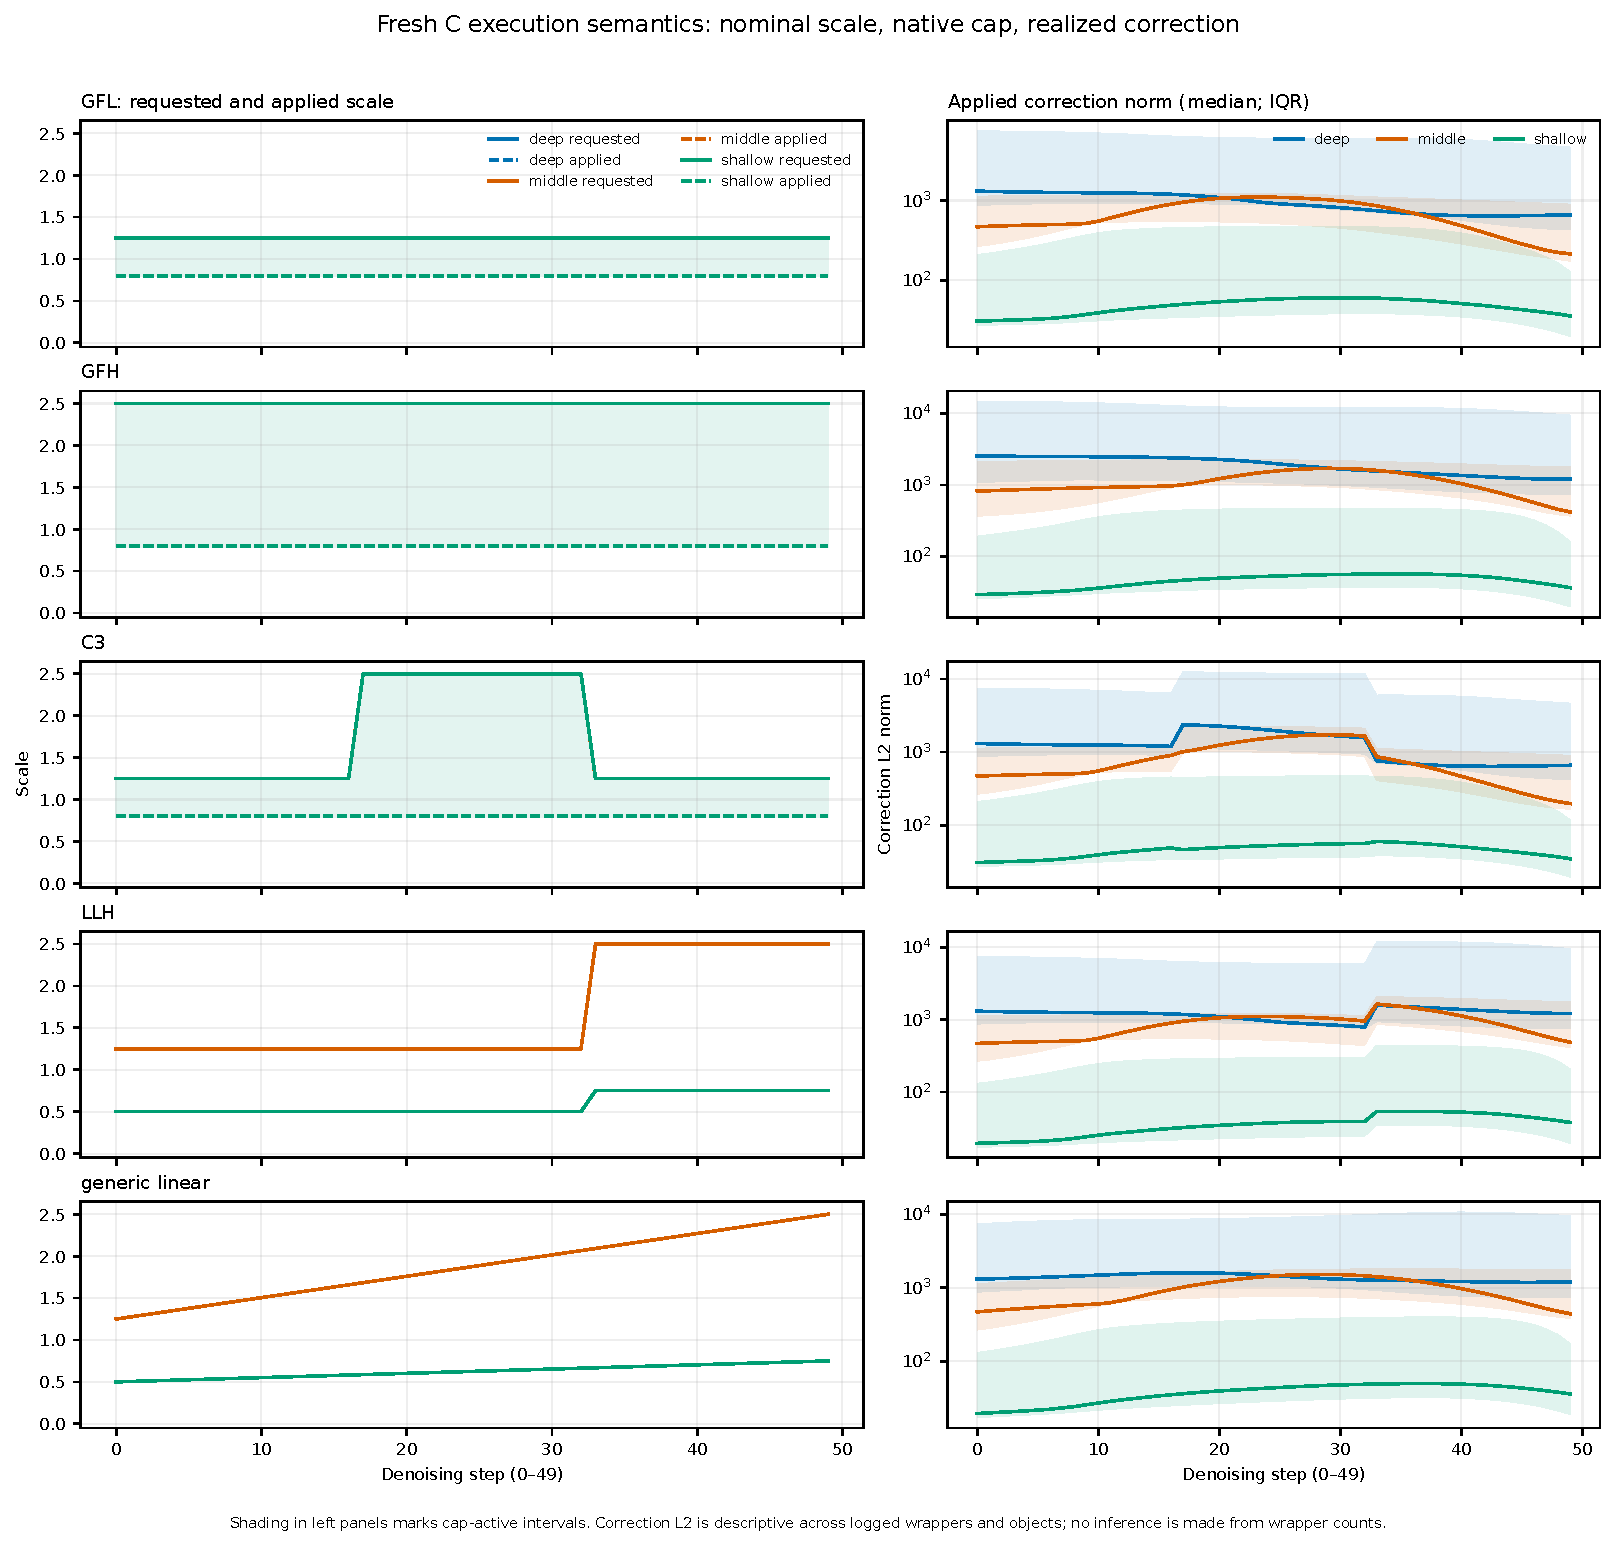
\includegraphics[width=0.88\textwidth]{../1006/figures/FRESH_C_EXECUTION_SEMANTICS.pdf}
\caption{Fresh C implementation-aware scale accounting. Left: requested and applied profiles for five adapter configurations, including intervals where native layer caps are active. Right: median and interquartile range of logged correction L2 norms across recorded wrappers and objects. The correction norms are descriptive; they do not define equal realized-dose interventions or explain image quality causally.}
\label{fig:execution}
\end{figure*}

\subsection{Fresh C Object-Level Results}
\label{subsec:freshc}

\subsubsection{Primary C3--GFL contrast}

For the Fresh C primary endpoint, the paired C3--GFL difference in foreground PSNR is +0.522 dB (95\% object-bootstrap CI [+0.404, +0.641]); the median object difference is +0.555 dB, and 68.7\% of objects favor C3 on this endpoint. This is a result for one specified image-space endpoint and comparator. Figure~\ref{fig:freshc_primary} shows its object-level distribution and uncertainty. The full endpoint table is provided in the supplementary material.

\begin{figure*}[t]
\centering
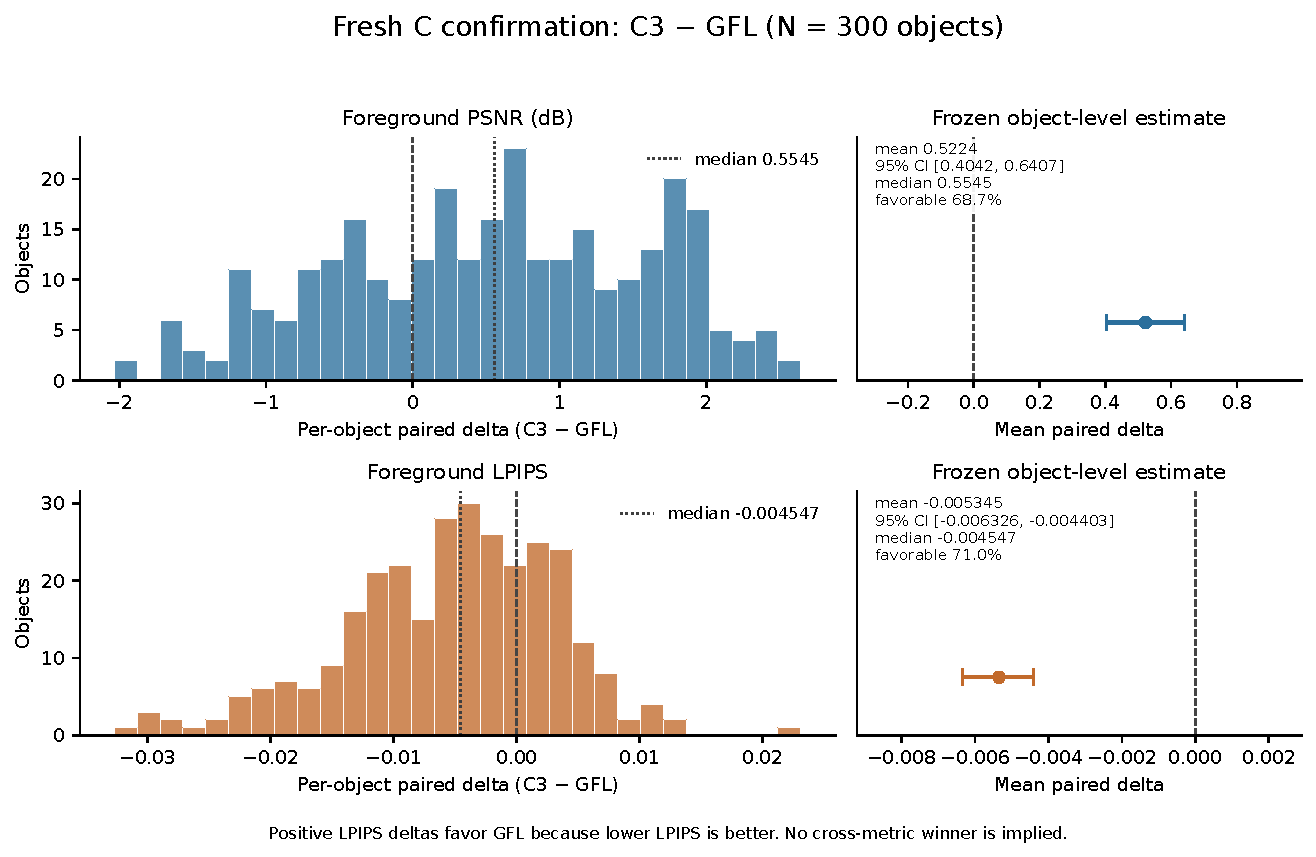
\includegraphics[width=0.78\textwidth]{../1006/figures/final_candidate/FIGURE_B_FRESH_C_C3_GFL.pdf}
\caption{Fresh C primary C3--GFL paired results for foreground PSNR and foreground LPIPS (N=300 objects). Histograms show paired object differences; point intervals show mean differences and 95\% object-bootstrap intervals. Positive LPIPS differences favor GFL because lower LPIPS is better.}
\label{fig:freshc_primary}
\end{figure*}

\subsubsection{Generic-linear and high-fixed-scale comparisons}

The separate Fresh C addendum shows endpoint- and object-level heterogeneity. For C3 minus generic linear, mean foreground PSNR is $-0.593$ dB (95\% CI $[-0.837,-0.351]$), which favors generic linear on the mean; the median is $+0.074$ dB and 51.7\% of objects favor C3, so the mean does not describe a typical-object advantage. For foreground LPIPS, C3 minus generic linear is $+0.01351$ (95\% CI $[+0.01160,+0.01549]$), favoring generic linear, with 25.7\% of objects favoring C3. Figure~\ref{fig:freshc_tradeoffs} shows the paired addendum distributions. These addendum contrasts are kept separate from the primary C3--GFL result.

The reviewer-requested C3--GFH analysis is \texttt{POST\_HOC WITHIN FROZEN FRESH-C COHORT}. For Edge-SSIM, C3 minus GFH is $-0.01881$ (95\% CI $[-0.02080,-0.01679]$); 47 of 300 objects favor C3 and one is tied, so this endpoint favors GFH. For full-image PSNR, the difference is $+0.6607$ dB (95\% CI $[+0.5858,+0.7358]$), with 252 of 300 objects favoring C3. This is an endpoint-specific trade-off. No non-inferiority margin was prespecified, and neither an interval crossing zero nor any other result is interpreted as equivalence or non-inferiority. The complete seven-endpoint table is reported in the supplement.

\begin{figure*}[t]
\centering
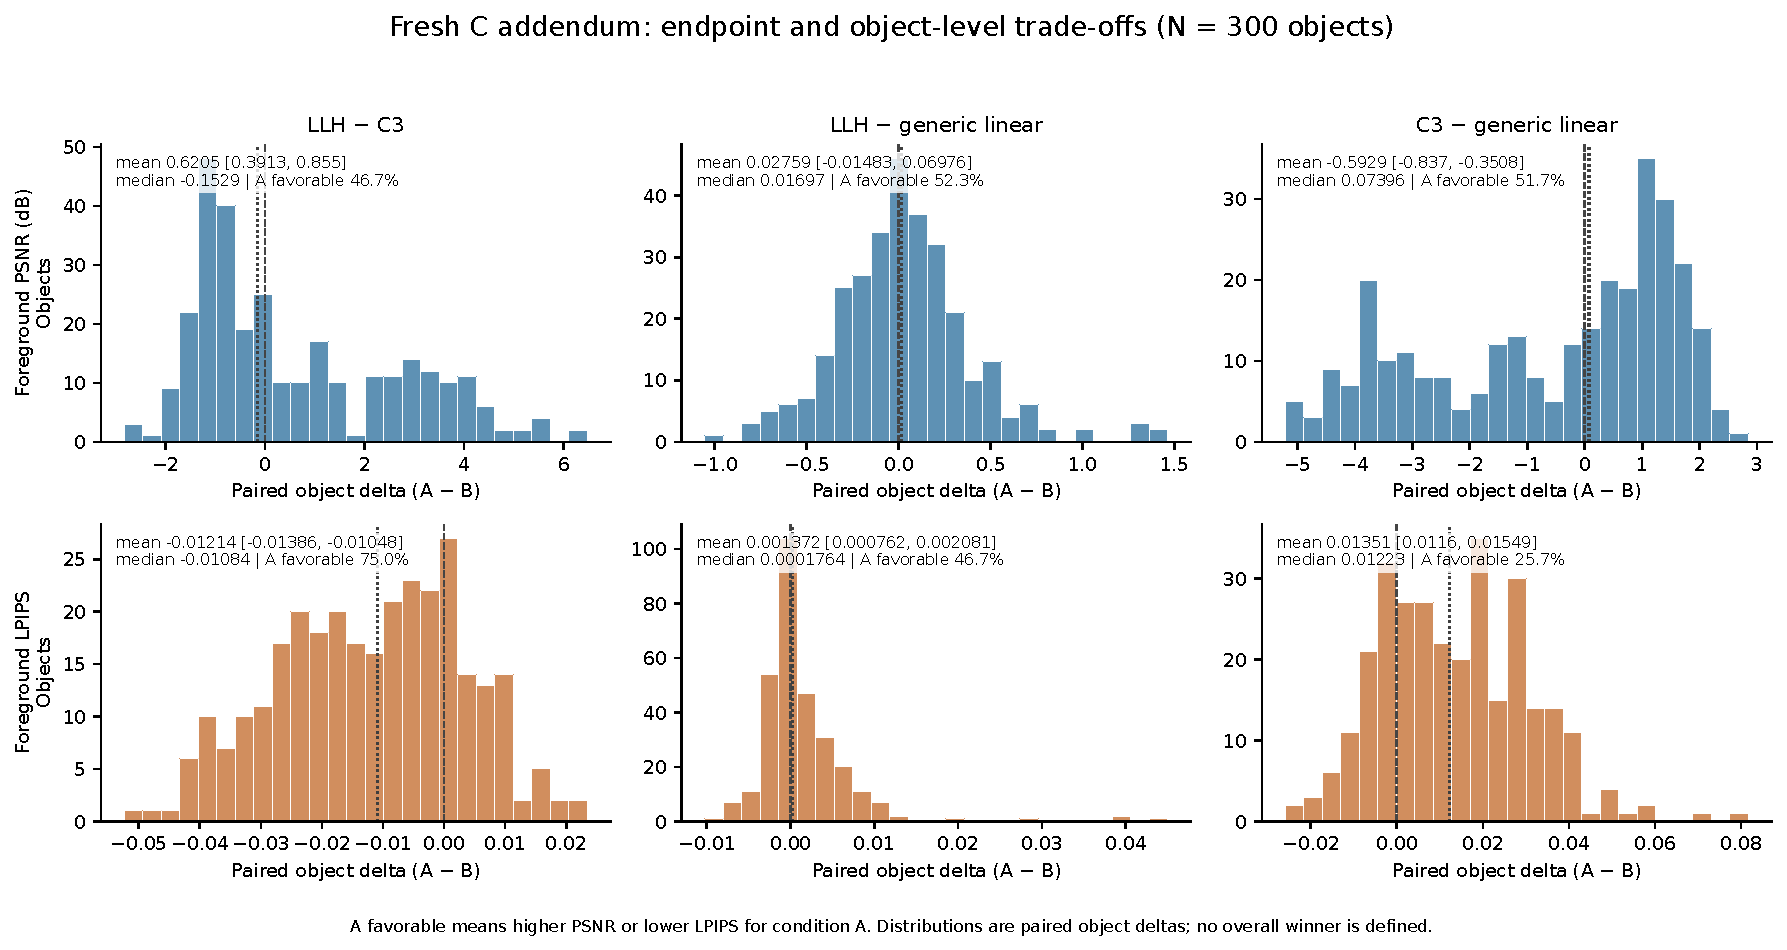
\includegraphics[width=0.94\textwidth]{../1006/figures/final_candidate/FIGURE_C_FRESH_C_TRADEOFFS.pdf}
\caption{Fresh C addendum paired object-level foreground PSNR and LPIPS differences for LLH, C3, and generic linear (N=300). Positive PSNR differences favor the first-named condition; lower LPIPS is better. These distributions illustrate endpoint and object heterogeneity and do not define an aggregate winner.}
\label{fig:freshc_tradeoffs}
\end{figure*}

\subsubsection{Selected qualitative illustrations}

Figure~\ref{fig:qualitative} presents selected, rights-cleared examples with the same reference views, camera, and layout across the compared conditions. The panels were curated to make method-specific differences easy to inspect, including a high C3--GFL foreground-PSNR case and a C3--generic-linear case with a visible trade-off. They are illustrations rather than a statistical sample; all cohort-level conclusions above use the complete frozen Fresh C cohort. Material and color discrepancies remain visible in selected outputs, including outputs with favorable image-space metrics.

\begin{figure*}[t]
\centering
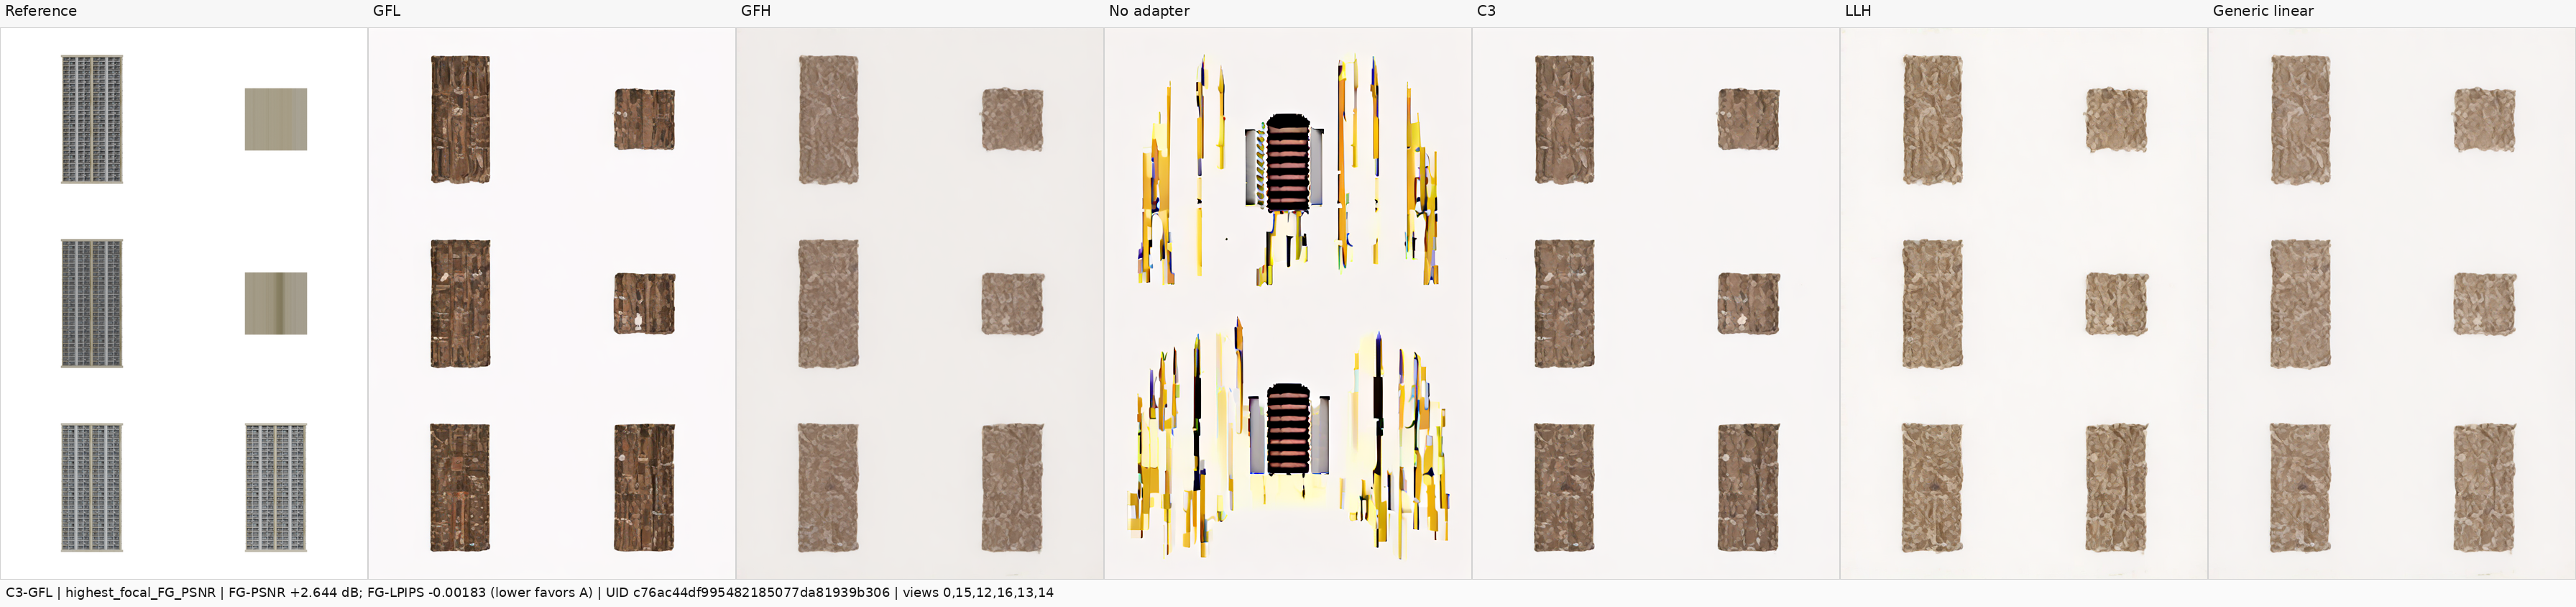
\includegraphics[width=0.96\textwidth]{../1006/review/REVIEWER_VISUAL_CANDIDATE_POOL/panels/candidate_01_c76ac44df995482185077da81939b306.png}\\[3pt]
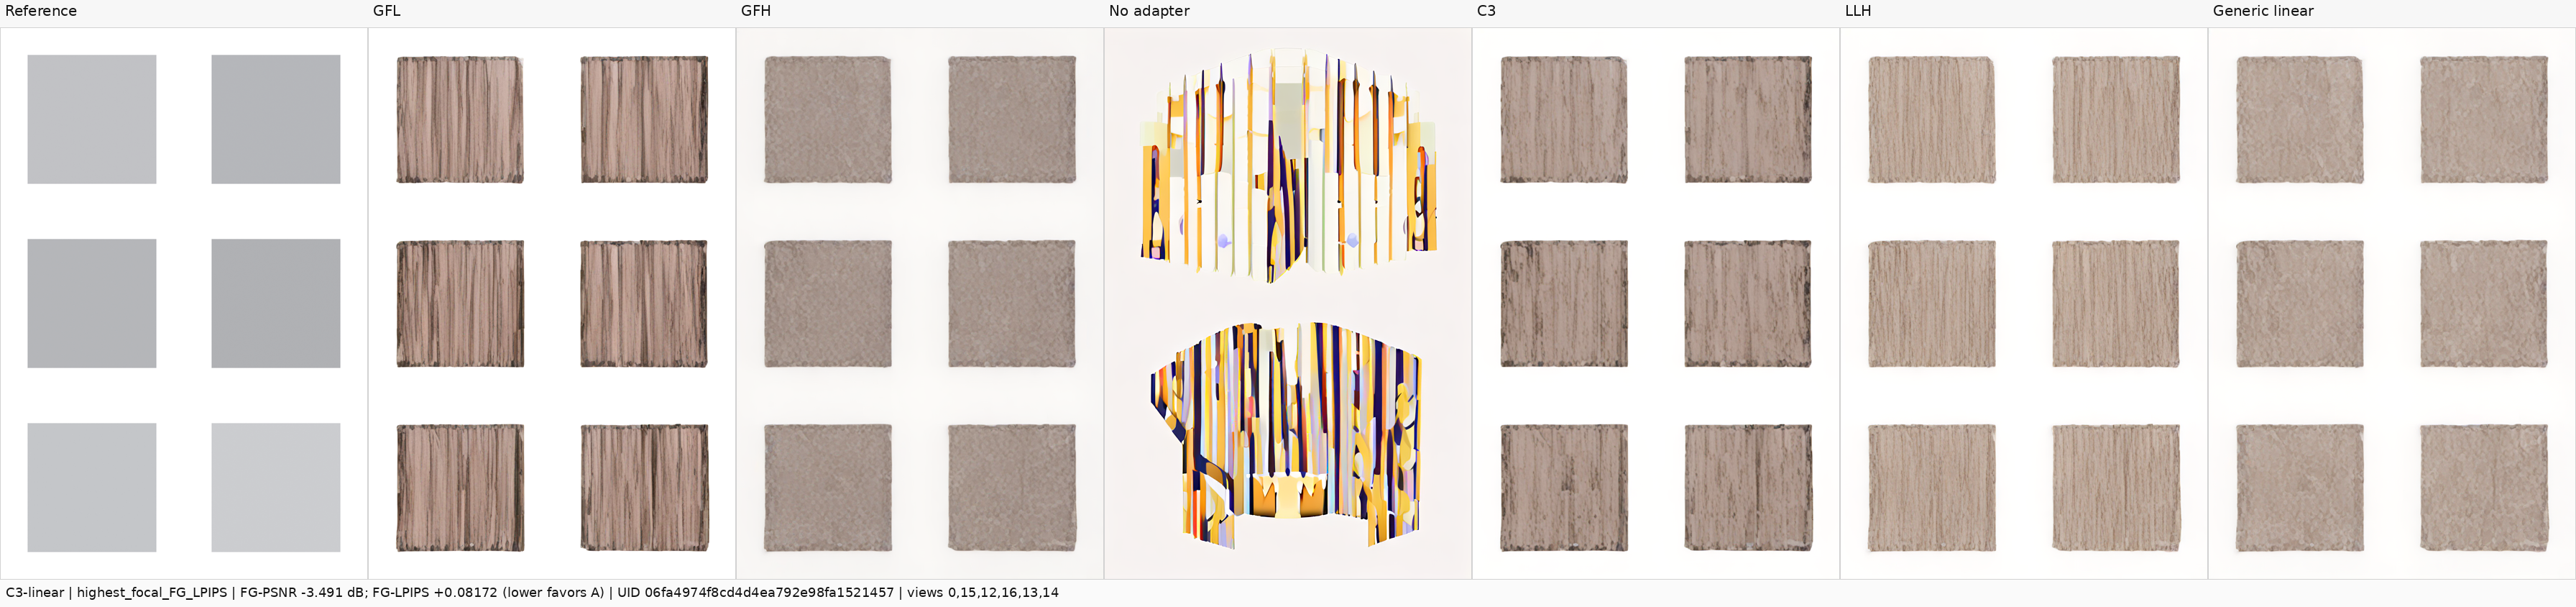
\includegraphics[width=0.96\textwidth]{../1006/review/REVIEWER_VISUAL_CANDIDATE_POOL/panels/candidate_20_06fa4974f8cd4d4ea792e98fa1521457.png}
\caption{Selected qualitative examples illustrating method-specific image-space behavior. Each row shows the reference and the same views for GFL, GFH, no adapter, C3, LLH, and generic linear. Examples were selected for visual clarity and reviewer relevance, not as a representative sample of the cohort. The first row is a high C3--GFL foreground-PSNR case; the second illustrates a C3--generic-linear trade-off. Quantitative conclusions are based on the full N=300 cohort.}
\label{fig:qualitative}
\end{figure*}

\subsection{Boundary Tests on Other Conditioning Interfaces}
\label{subsec:boundary}

The MVDiffusion and MV-Adapter studies are interface-specific boundary tests, not matched replications of the GeoTex residual-adapter intervention. MVDiffusion applies schedules through correspondence-aware decoder-side CPBlocks. In its 75-object panel, the official SD2-depth weights were unavailable, so all within-panel conditions used the same compatibility base. For the layer-wise LLH versus global linear comparison, the mean PSNR difference is $-0.454$ dB (95\% CI $[-0.752,-0.161]$), while the FG-LPIPS difference is $-0.0027$ (95\% CI $[-0.0076,+0.0018]$); the measured endpoints therefore do not show a uniform direction of benefit. MV-Adapter uses a different additive-residual interface; 98 objects remained after one source-mesh exclusion. Its exploratory interaction reanalysis found no metric surviving Holm correction, so the study does not confirm the broad interaction observed on the primary system; this is not evidence that interaction is absent. We do not pool outcomes across interfaces or infer architecture-level causes. These results bound the tested transfer claims and leave broader transfer unestablished.

\section{Limitations}
\label{sec:limitations}

This study measures one existing geometry-conditioned adapter implementation under a fixed pipeline, checkpoint, sampler, and set of target views. The requested-to-applied-scale mapping and correction magnitudes are implementation-specific. The comparisons do not normalize realized residual dose and do not establish a causal effect of correction norm on image outcomes.

The quantitative endpoints are image-space similarities and local variation statistics. They do not establish material correctness, perceptual preference, quality on unseen views, baked-texture quality, or seam consistency. Selected figures are qualitative illustrations only. The 300-object Fresh C cohort is a revision-era follow-up motivated by earlier results, not an independent replication under the original registration; conclusions should therefore remain tied to this frozen cohort and its tested conditions.

The additional MVDiffusion and MV-Adapter tests use different conditioning interfaces and are not matched replications. The MVDiffusion panel used a compatibility base because the official depth weights were unavailable; the exploratory MV-Adapter interaction analysis did not confirm the broad response pattern observed on the primary system. These boundary tests do not establish universal transfer, nor do they prove that transfer is absent. Broader evaluation across implementations and independently assembled cohorts remains future work.

\section{Conclusion}
\label{sec:conclusion}

We report an implementation-aware analysis of adapter scaling in one geometry-controlled multi-view diffusion pipeline. In the evaluated wrapper, requested scales pass through layer-specific rules and caps, and the applied correction magnitude also depends on the residual being scaled. A nominal scale therefore does not specify an equal realized intervention.

On the frozen Fresh C cohort of 300 objects, the primary C3--GFL foreground-PSNR difference is +0.522 dB (95\% object-bootstrap CI [+0.404, +0.641]), with 68.7\% of objects favoring C3 on that endpoint. In a separate addendum, generic linear has higher mean foreground PSNR and lower mean foreground LPIPS than C3, while object-level results are heterogeneous. The post-hoc C3--GFH comparison also shows an Edge-SSIM cost alongside a full-image PSNR advantage. These findings support endpoint-specific reporting, not a single overall winner.

The paper's contribution is limited to measured execution semantics and object-level image-space evidence for the tested implementation and configurations. It does not introduce a new scheduling primitive, derive an optimum, establish cross-interface transfer, or claim general perceptual, material, baked-texture, or seam fidelity.

\section*{Data availability}

All data included in this study are available upon request by contact with the corresponding author.

\section*{Declaration of competing interests}

The authors declare that they have no known competing financial interests or personal relationships that could have appeared to influence the work reported in this paper.


\begin{thebibliography}{47}
\bibitem{liu2023zero1to3}
Liu R, Wu R, Van Hoorick B, et al. Zero-1-to-3: Zero-shot one image to 3D object. \textit{Proceedings of the IEEE/CVF International Conference on Computer Vision}, 2023.

\bibitem{shi2023zero123pp}
Shi R, Chen H, Zhang Z, et al. Zero123++: A single image to consistent multi-view diffusion base model. arXiv:2310.15110, 2023.

\bibitem{liu2023syncdreamer}
Liu Y, Lin C, Zeng Z, et al. SyncDreamer: Generating multiview-consistent images from a single-view image. \textit{International Conference on Learning Representations}, 2024.

\bibitem{long2023wonder3d}
Long X, Guo Y C, Lin C, et al. Wonder3D: Single image to 3D using cross-domain diffusion. \textit{Proceedings of the IEEE/CVF Conference on Computer Vision and Pattern Recognition}, 2024.

\bibitem{shi2024mvdream}
Shi Y, Wang P, Ye J, et al. MVDream: Multi-view diffusion for 3D generation. \textit{International Conference on Learning Representations}, 2024.

\bibitem{wang2023imagedream}
Wang P, et al. ImageDream: Image-prompt multi-view diffusion for 3D generation. arXiv:2312.02201, 2023.

\bibitem{xu2024instantmesh}
Xu J, et al. InstantMesh: Efficient 3D mesh generation from a single image with sparse-view large reconstruction models. \textit{Advances in Neural Information Processing Systems}, 2024.

\bibitem{ke2024era3d}
Li P, Liu Y, Long X, et al. Era3D: High-resolution multiview diffusion using efficient row-wise attention. \textit{Advances in Neural Information Processing Systems}, 2024.

\bibitem{chen2023text2tex}
Chen D Z, et al. Text2Tex: Text-driven texture synthesis via diffusion models. \textit{Proceedings of the IEEE/CVF International Conference on Computer Vision}, 2023.

\bibitem{richardson2023texture}
Richardson E, Metzer G, Alaluf Y, et al. TEXTure: Text-guided texturing of 3D shapes. \textit{ACM SIGGRAPH 2023 Conference Proceedings}, 2023.

\bibitem{poole2023dreamfusion}
Poole B, Jain A, Barron J T, Mildenhall B. DreamFusion: Text-to-3D using 2D diffusion. \textit{International Conference on Learning Representations}, 2023.

\bibitem{chen2023fantasia3d}
Chen R, Chen Y, Jiao N, Jia K. Fantasia3D: Disentangling geometry and appearance for high-quality text-to-3D content creation. \textit{Proceedings of the IEEE/CVF International Conference on Computer Vision}, 2023.

\bibitem{shao2025mvpainter}
Shao M, Xiong F, Sun Z, Xu M. MVPainter: Accurate and detailed 3D texture generation via multi-view diffusion with geometric control. arXiv:2505.12635, 2025.

\bibitem{kynkanniemi2024limited}
Kynk\"a\"anniemi T, Aittala M, Karras T, et al. Applying guidance in a limited interval improves sample and distribution quality in diffusion models. \textit{Advances in Neural Information Processing Systems}, 2024.

\bibitem{kulkarni2026ssi}
Kulkarni A S. Scheduled Style Injection: Expanding the Style-Content Pareto Frontier in Training-Free Diffusion-based Style Transfer. In: \textit{Proceedings of the IEEE/CVF Conference on Computer Vision and Pattern Recognition Workshops (NTIRE)}, 2026.

\bibitem{papalampidi2025dynamiccfg}
Papalampidi P, Wiles O, Ktena I, et al. Dynamic Classifier-Free Diffusion Guidance via Online Feedback. arXiv:2509.16131, 2025.

\bibitem{perla2026survey}
Perla S R K, Zhang H, Mahdavi-Amiri A. Advances in neural 3D mesh texturing: A survey. \textit{Computer Graphics Forum}, 2026, e70392.

\bibitem{guzman2026adaptive}
Guzm\'an J E, Mould D, Paquette E. Adaptive multiresolution exemplar-based texture synthesis on animated fluids. \textit{Computers \& Graphics}, 2026, 134: 104490.

\bibitem{lv2025interpretable}
Lv X, Wu Z, Xu J, et al. Interpretable procedural material graph generation via diffusion models from reference images. \textit{The Visual Computer}, 2025, 41(13): 11195--11205.

\bibitem{zeng2024paint3d}
Zeng X, Chen X, Qi Z, et al. Paint3D: Paint anything 3D with lighting-immersive texture generation. \textit{Proceedings of the IEEE/CVF Conference on Computer Vision and Pattern Recognition}, 2024.

\bibitem{cheng2024mvpaint}
Cheng W, Mu J, Zeng X, et al. MVPaint: Synchronized multi-view diffusion for painting anything 3D. \textit{Proceedings of the IEEE/CVF Conference on Computer Vision and Pattern Recognition}, 2025.

\bibitem{lai2025hunyuan3d}
Zhao Z, Lai Z, Lin Q, et al. Hunyuan3D 2.0: Scaling diffusion models for high resolution textured 3D assets generation. arXiv:2501.12202, 2025.

\bibitem{huang2024mvadapter}
Huang Z, et al. MV-Adapter: Multi-view consistent image generation made easy. \textit{Proceedings of the IEEE/CVF International Conference on Computer Vision}, 2025.

\bibitem{liu2024synchronized}
Liu Y X, Xie M S, Liu H Y, Wong T T. Text-guided texturing by synchronized multi-view diffusion. \textit{SIGGRAPH Asia 2024 Conference Papers}, 2024.

\bibitem{xu2026wondertex}
Xu Q, Han X G, Zhang L. WonderTex: Consistent-and-seamless texture generation with text-guided multi-view image diffusion models. \textit{IEEE Transactions on Visualization and Computer Graphics}, 2026, 32(7): 5815--5825.

\bibitem{mou2023t2iadapter}
Mou C, Wang X, Xie L, et al. T2I-Adapter: Learning adapters to dig out more controllable ability for text-to-image diffusion models. \textit{Proceedings of the AAAI Conference on Artificial Intelligence}, 2024.

\bibitem{zhang2023controlnet}
Zhang L, Rao A, Agrawala M. Adding conditional control to text-to-image diffusion models. \textit{Proceedings of the IEEE/CVF International Conference on Computer Vision}, 2023.

\bibitem{ye2023ipadapter}
Ye H, Zhang J, Liu S, Han X, Yang W. IP-Adapter: Text compatible image prompt adapter for text-to-image diffusion models. arXiv:2308.06721, 2023.

\bibitem{hu2022lora}
Hu E J, Shen Y, Wallis P, et al. LoRA: Low-rank adaptation of large language models. \textit{International Conference on Learning Representations}, 2022.

\bibitem{liu2024dora}
Liu S Y, Wang C Y, Yin H, et al. DoRA: Weight-decomposed low-rank adaptation. \textit{International Conference on Machine Learning}, 2024.

\bibitem{zhang2023adalora}
Zhang Q, Zuo S, Liang C, et al. AdaLoRA: Adaptive budget allocation for parameter-efficient fine-tuning. \textit{International Conference on Learning Representations}, 2023.

\bibitem{ho2020ddpm}
Ho J, Jain A, Abbeel P. Denoising diffusion probabilistic models. \textit{Advances in Neural Information Processing Systems}, 2020.

\bibitem{song2021ddim}
Song J, Meng C, Ermon S. Denoising diffusion implicit models. \textit{International Conference on Learning Representations}, 2021.

\bibitem{ho2022cfg}
Ho J, Salimans T. Classifier-free diffusion guidance. \textit{NeurIPS Workshop on Deep Generative Models and Downstream Applications}, 2021. arXiv:2207.12598.

\bibitem{castillo2023adaptive}
Castillo A, Kohler J, P\'erez J C, et al. Adaptive guidance: Training-free acceleration of conditional diffusion models. \textit{Proceedings of the AAAI Conference on Artificial Intelligence}, 2025.

\bibitem{rombach2022ldm}
Rombach R, Blattmann A, Lorenz D, Esser P, Ommer B. High-resolution image synthesis with latent diffusion models. \textit{Proceedings of the IEEE/CVF Conference on Computer Vision and Pattern Recognition}, 2022.

\bibitem{esser2024scaling}
Esser P, Kulal S, Blattmann A, et al. Scaling rectified flow transformers for high-resolution image synthesis. \textit{International Conference on Machine Learning}, 2024.

\bibitem{blackforestlabs2024flux}
Black Forest Labs. FLUX: Flow matching for image generation. https://github.com/black-forest-labs/flux, 2024.

\bibitem{loshchilov2019decoupled}
Loshchilov I, Hutter F. Decoupled weight decay regularization. \textit{International Conference on Learning Representations}, 2019.

\bibitem{cherti2023reproducible}
Cherti M, Beaumont R, Wightman R, et al. Reproducible scaling laws for contrastive language-image learning. \textit{Proceedings of the IEEE/CVF Conference on Computer Vision and Pattern Recognition}, 2023.

\bibitem{nichol2022glide}
Nichol A, Dhariwal P, Ramesh A, et al. GLIDE: Towards photorealistic image generation and editing with text-guided diffusion models. \textit{International Conference on Machine Learning}, 2022.

\bibitem{saharia2022photorealistic}
Saharia C, Chan W, Saxena S, et al. Photorealistic text-to-image diffusion models with deep language understanding. \textit{Advances in Neural Information Processing Systems}, 2022.

\bibitem{peebles2023scalable}
Peebles W, Xie S. Scalable diffusion models with transformers. \textit{Proceedings of the IEEE/CVF International Conference on Computer Vision}, 2023.

\bibitem{wang2004ssim}
Wang Z, Bovik A C, Sheikh H R, Simoncelli E P. Image quality assessment: From error visibility to structural similarity. \textit{IEEE Transactions on Image Processing}, 2004, 13(4): 600--612.

\bibitem{zhang2018lpips}
Zhang R, Isola P, Efros A A, Shechtman E, Wang O. The unreasonable effectiveness of deep features as a perceptual metric. \textit{Proceedings of the IEEE/CVF Conference on Computer Vision and Pattern Recognition}, 2018.

\bibitem{wang2023clipiqa}
Wang J, Chan K C K, Loy C C. Exploring CLIP for assessing the look and feel of images. \textit{Proceedings of the AAAI Conference on Artificial Intelligence}, 2023.

\bibitem{radford2021clip}
Radford A, Kim J W, Hallacy C, et al. Learning transferable visual models from natural language supervision. \textit{International Conference on Machine Learning}, 2021.

\end{thebibliography}
\end{document}
